\documentclass[conference]{IEEEtran}
\usepackage{graphicx}
\usepackage{url}

\begin{document}

\title{Phishing Email Detection with Tuned Classical Machine Learning Models:\\A Leakage-Aware Study on a Combined Public Corpus}

\author{
\IEEEauthorblockN{Thirugnanam V S}
\IEEEauthorblockA{School of Electronics Engineering (SENSE)\\
Vellore Institute of Technology, Chennai, India}
}

\maketitle

\begin{abstract}
Phishing remains the most common entry point for email-borne attacks, and
public benchmark corpora make the detection task look close to solved. In
this work, carried out as part of the IICT summer internship on AI and
machine learning, we build a complete phishing email classifier from
scratch on a widely used combined corpus of 82{,}486 emails and examine
what the resulting scores actually measure. The corpus arrives partially
normalised; we verify this claim empirically (0.0\% of emails contain
uppercase or HTML remnants, while 47.2\% still carry URL tokens), remove
a measured source watermark (the token \textit{enron} appears in 18.2\%
of legitimate emails and 0.0\% of phishing ones), truncate 255 extreme
outliers, and de-duplicate 409 rows before any model sees the data. Four
classifiers required by the project brief are compared on identical
TF-IDF features and an identical stratified split, with grid-searched
hyperparameters where the search is compute-cheap. Tuned logistic
regression ($C=10$) performs best with 98.22\% accuracy, an F1 score of
0.9829 and --- most importantly for this domain --- a recall of 0.9851,
missing 128 of 8{,}569 phishing emails in the held-out test set.
Inspecting the learned weights shows that alongside genuine phishing
vocabulary, several of the strongest features are names of the source
archives themselves, which we argue is the correct lens for interpreting
near-ceiling results on combined corpora.
\end{abstract}

\begin{IEEEkeywords}
phishing detection, email security, text classification, machine
learning, TF-IDF, data leakage, hyperparameter tuning
\end{IEEEkeywords}

\section{Introduction}
Phishing emails try to manoeuvre a recipient into clicking a link,
opening an attachment or replying with credentials, and filtering them
automatically has been studied since the mid-2000s
\cite{fette2007,almomani2013}. Public datasets make it easy to train a
classifier that scores in the high nineties --- and easy to stop asking
what the classifier learned. This paper documents an end-to-end pipeline
built during the IICT summer internship with the opposite emphasis:
every preprocessing decision is justified by a measurement taken from
the data, the feature representation is chosen by a pre-declared
protocol rather than by habit, and the final analysis reads the winning
model's weights to separate genuine phishing signal from dataset
artefact.

The contributions are practical: (i) a verify-then-apply preprocessing
pass that measures, rather than assumes, what cleaning the corpus still
needs, and removes a quantified source watermark; (ii) a controlled
comparison of the four models required by the project brief --- logistic
regression, multinomial naive Bayes, random forest and a multi-layer
perceptron --- on identical features and splits, with grid-searched
hyperparameters where the search is cheap and a written rationale where
it is not; (iii) a recall-first reading of the results, since a missed
phishing email costs a user far more than a false alarm costs a
reviewer; and (iv) an inspection of the learned coefficients that names,
concretely, which top features are corpus watermarks. All numbers in
this paper were produced by the accompanying code from a single seeded
run; nothing is quoted from other papers as our own result.

\section{Related Work}
Fette et al. framed phishing detection as machine learning over email
features and reported strong results with a random-forest-style
classifier \cite{fette2007}. Almomani et al. survey the filtering
literature and catalogue the feature families --- textual, URL-based and
header-based --- that later systems draw on \cite{almomani2013}. On the
data side, the Enron corpus \cite{klimt2004} became the standard source
of legitimate business email, and Metsis et al. built the widely used
Enron-Spam benchmarks by pairing it with spam collections
\cite{metsis2006}. The corpus used here continues that tradition:
it aggregates ham from Enron-era mailboxes and public mailing lists with
phishing and scam messages from public archives. That construction is
precisely why Section~VI-B matters: when each class comes from different
archives, part of any classifier's accuracy is archive recognition.

\section{Dataset and Cleaning}
\subsection{Raw Data}
The dataset is a single CSV of 82{,}486 emails with two columns:
\textit{text\_combined} (subject and body merged by the dataset authors)
and a binary label --- 42{,}891 phishing (label 1) and 39{,}595
legitimate (label 0), a comfortable 52/48 balance. No values are
missing. Label semantics were verified by sampling rather than assumed:
label-1 emails read like promotions and scams, label-0 emails like
internal business mail.

\subsection{Verify-Then-Apply Preprocessing}
The text arrives partially normalised by the dataset authors, and the
right engineering response is to measure that claim. Our inspection code
found uppercase letters in 0.0\% of emails and HTML remnants in 0.0\% ---
but URL fragments (\textit{http}) still in 47.2\% and digits in 94.2\%.
The standard normalisation pipeline (URL and HTML removal, non-letter
stripping, English stop words) therefore still earns its place, and the
inspection report is the evidence. One consequence is recorded honestly:
upstream normalisation already destroyed URL \textit{structure}, so
URL-based features can only be approximated at the token level.

\subsection{Source Watermark}
A large share of the legitimate class descends from the Enron corpus
\cite{klimt2004}, and it shows: the token \textit{enron} appears in
18.2\% of legitimate emails and 0.0\% of phishing ones. A company name
is not phishing signal --- it is a label for where the ham was collected
--- so \textit{enron} was added to the stop-word list, for the same
reason a news-agency dateline would be stripped in a fake-news task.
Deeper source effects that single tokens cannot capture are measured in
Section~VI-B.

\subsection{Duplicates, Conflicts and Outliers}
Extreme lengths were handled first: the longest raw email runs
4{,}279{,}526 characters (median 558) --- a mailing-list digest --- so
emails are truncated at 20{,}000 characters, which touched 255 messages
(0.31\% of the data) while keeping every email's informative opening.
Truncation runs \textit{before} de-duplication on purpose: two long
emails that differ only beyond the cap become identical afterwards, and
de-duplication must operate on the text the models will actually see.
In total 409 exact duplicate rows were removed; a dedicated check for
texts appearing under both labels found none (no labelling conflicts in
this corpus); one empty email and one digits-only email were dropped.
The final corpus holds 82{,}075 emails: 42{,}843 phishing and 39{,}232
legitimate (52.2\% phishing).

\subsection{Exploratory Findings}
Legitimate emails average 168 words after preprocessing (median 93,
s.d.~260) against 103 for phishing (median 48, s.d.~156); both
distributions pile up on short messages and overlap heavily, so length
alone cannot separate the classes. The vocabularies, however, barely
overlap: only 7 of the top-20 words are shared between classes, with
workplace and scheduling vocabulary on one side and promotional, action
vocabulary on the other. Fig.~\ref{fig:keywords} makes the same point
with a fixed list of fifteen classic scam words chosen \textit{before}
looking at the data: every one occurs more often in phishing ---
\textit{click} leads at 14.7\% of phishing emails against 4.8\% of
legitimate, and \textit{money} shows the widest gap (14.4\% vs 2.6\%)
--- yet none is remotely universal, which is exactly why the models use
5{,}000 word features instead of a keyword rule.

\begin{figure}[t]
\centering
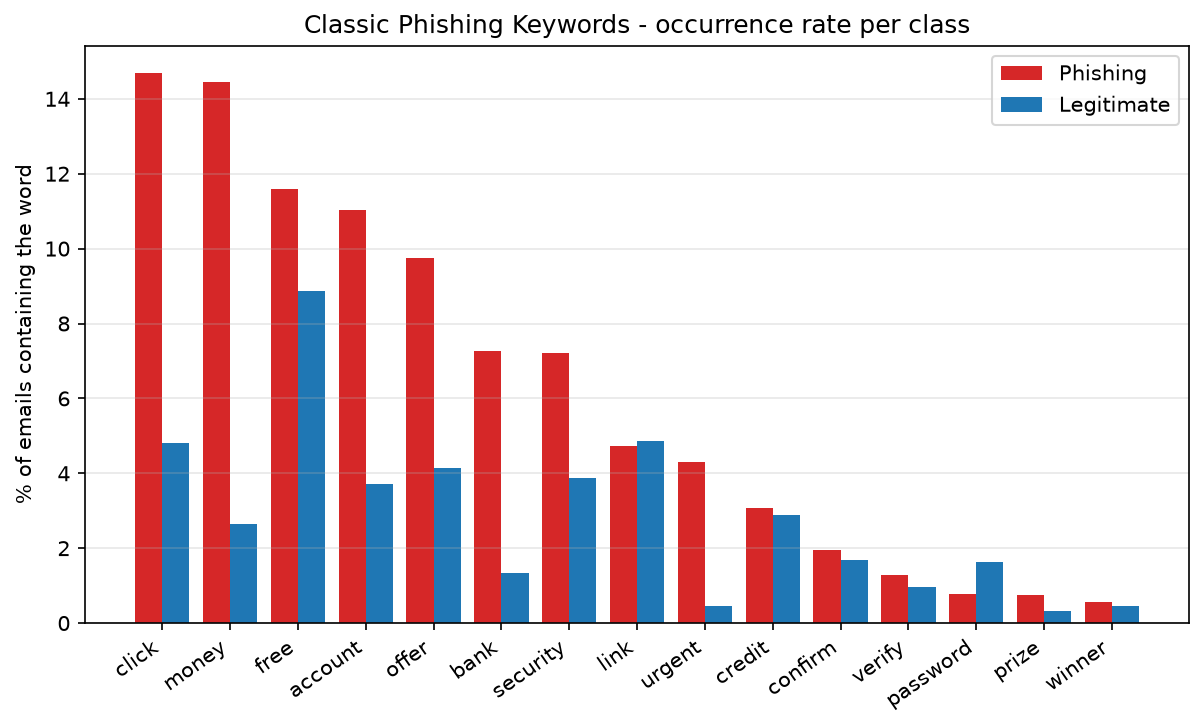
\includegraphics[width=\columnwidth]{figs/phishing_keywords.png}
\caption{Occurrence rate of fifteen classic scam keywords per class. The
list was fixed before inspecting the data.}
\label{fig:keywords}
\end{figure}

\section{Methodology}
\subsection{Split and Features}
The cleaned corpus was split 80/20 with stratification on the label and
a fixed seed (42), giving 65{,}660 training and 16{,}415 testing emails
with an identical 52.2\% phishing share on both sides. All feature
extraction was fitted on the training portion only.

Raw term counts and TF-IDF weighting were compared with an identical
logistic regression probe under 3-fold cross-validation on the training
set, both limited to the 5{,}000 most frequent terms. The result was a
statistical tie: counts scored a mean CV F1 of 0.9805 ($\pm$0.0013)
against 0.9801 ($\pm$0.0010) for TF-IDF, a gap of 0.0003 --- inside the
0.001 tie threshold declared before the comparison was run. The
pre-declared tie rule selects TF-IDF: it down-weights near-universal
words, and it is the representation suggested by the project brief. We
note the value of running the comparison anyway: in a companion project
on news text, the identical protocol produced a decisive win for raw
counts, so the ``obvious'' default is not always the measured winner.

\subsection{Models and Tuning}
Four classifiers were trained on the identical feature matrices:
logistic regression, multinomial naive Bayes, a random forest (100
trees) and a multi-layer perceptron (one hidden layer of 100 units,
Adam, early stopping with patience 5). Hyperparameters were grid-searched
where the search is compute-cheap and meaningful: 3-fold cross-validation
on the training set selected $C=10$ for logistic regression (from
0.1/1/10, CV F1 0.9827 against 0.9801 at the default) and
$\alpha=0.1$ for naive Bayes (from 0.1/0.5/1.0, CV F1 0.9605). The
forest stays at 100 trees --- forests are famously insensitive to adding
trees beyond this point --- and the early-stopped MLP self-regularises
by construction; the searched grids and winners are written to a tuning
table by the pipeline so the scope of the search is visible rather than
implied. Every stochastic model shares the project seed.

\subsection{Evaluation}
Models are compared on accuracy, precision, recall and F1, computed for
the phishing class, with one confusion matrix and one full
classification report per model. Recall receives particular attention in
the analysis: a false negative is a scam reaching an inbox.

\section{Results}
Table~\ref{tab:results} summarises the held-out test performance;
Fig.~\ref{fig:f1comp} shows the F1 comparison and
Fig.~\ref{fig:cm} the winner's confusion matrix.

\begin{table}[t]
\caption{Test-set performance (16{,}415 emails). P, R and F1 refer to the phishing class.}
\label{tab:results}
\centering
\begin{tabular}{l c c c c}
\hline
Model & Acc. & P & R & F1 \\
\hline
Logistic Regression ($C{=}10$) & \textbf{0.9822} & 0.9808 & \textbf{0.9851} & \textbf{0.9829} \\
MLP (100 units)                & 0.9818 & 0.9803 & 0.9849 & 0.9826 \\
Random Forest                  & 0.9814 & 0.9850 & 0.9792 & 0.9821 \\
Multinomial NB ($\alpha{=}0.1$)& 0.9567 & 0.9743 & 0.9419 & 0.9578 \\
\hline
\end{tabular}
\end{table}

\begin{figure}[t]
\centering
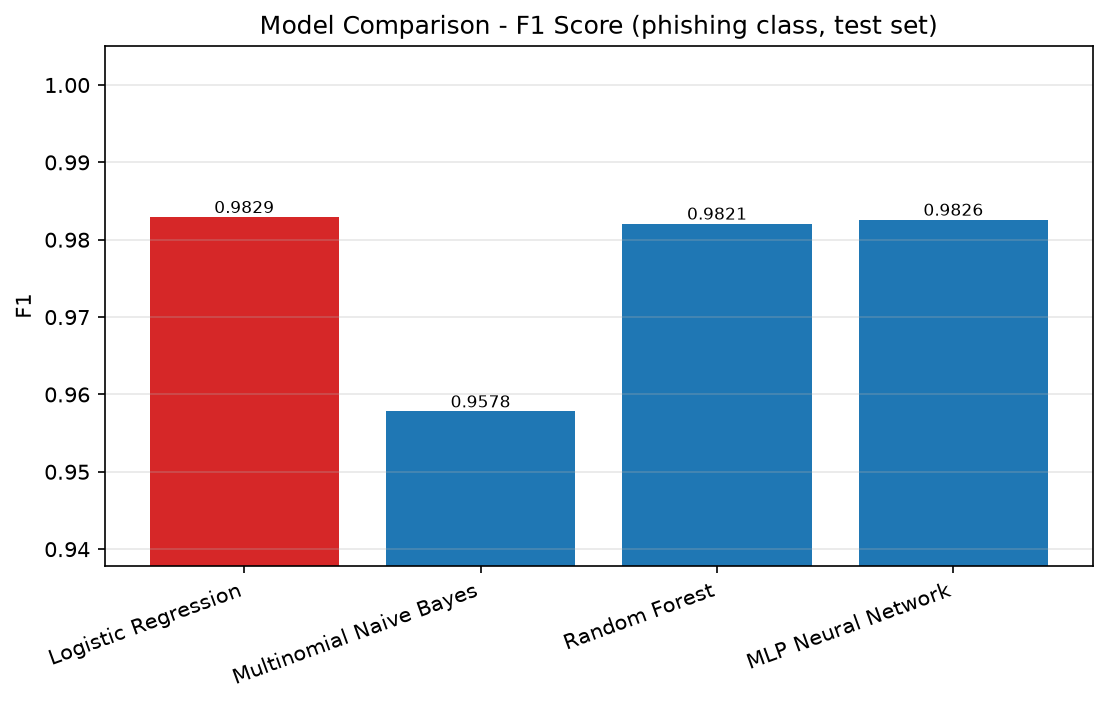
\includegraphics[width=\columnwidth]{figs/model_comparison_f1.png}
\caption{F1 score (phishing class) of the four models on the held-out
test set. The best model is highlighted.}
\label{fig:f1comp}
\end{figure}

\begin{figure}[t]
\centering
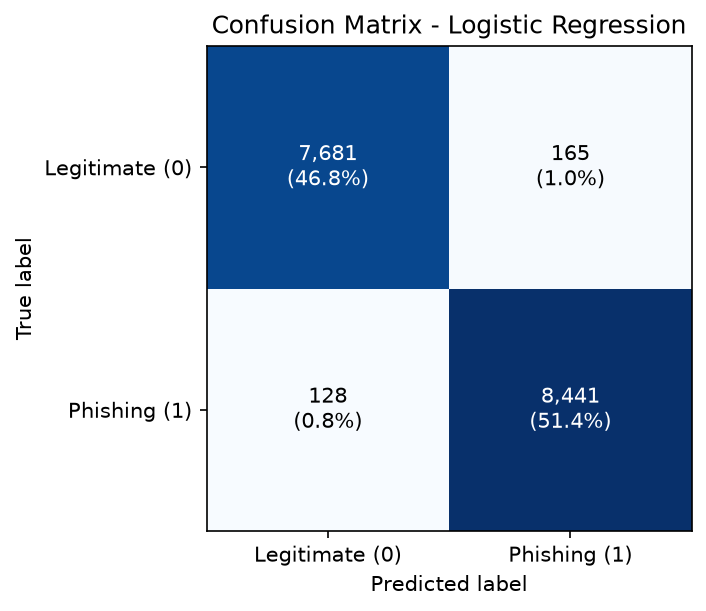
\includegraphics[width=0.85\columnwidth]{figs/confusion_matrix_logistic_regression.png}
\caption{Confusion matrix of the best model (tuned logistic regression).}
\label{fig:cm}
\end{figure}

Tuned logistic regression is the best model with 98.22\% accuracy, F1
0.9829 and recall 0.9851. Out of 16{,}415 test emails it makes 293
errors: 165 legitimate emails flagged as phishing and 128 phishing
emails missed --- about 15 misses per 1{,}000 phishing emails. The race
at the top is extraordinarily tight: the MLP (0.9826) and the random
forest (0.9821) sit within 0.0008 F1 of the winner. With vocabularies
this disjoint the classes are already close to linearly separable, so
the MLP's extra capacity mostly re-draws the same boundary at 46.6\,s of
training against 0.4\,s, and the forest's interaction modelling buys a
precision edge (0.9850, the best of the four) at the cost of the lowest
recall among the top three (0.9792) and 14.3\,s of training. Naive Bayes
trails at 0.9578 despite tuned smoothing; its recall of 0.9419 ---
498 missed phishing emails, nearly four times the winner's --- makes it
the wrong choice for this domain even where its speed appeals. Tuning
itself earned its keep twice: $\alpha=0.1$ beat the naive Bayes default,
and $C=10$ lifted the logistic regression probe's CV F1 from 0.9801 to
0.9827.

\section{Discussion}
\subsection{Recall First}
For phishing the two error types are not symmetric: a false positive
sends a legitimate email to a review folder, a false negative delivers a
scam. Ranking by F1 and reading recall alongside it, the tuned logistic
regression is the right pick twice over --- it tops both. Its 128 false
negatives are also informative as a group: the phishing emails it misses
average 180 words (median 70) against 104 words for phishing overall, so
the misses skew towards the longer messages that mix enough neutral
business vocabulary to blur the boundary, while short, punchy scams are
caught almost perfectly. Misclassified emails of both kinds are longer
than correctly classified ones on average (164 vs 133 words).

\subsection{What the Model Actually Learned}
Reading the strongest logistic-regression coefficients
(Fig.~\ref{fig:importance}) is sobering in the most useful way. On the
phishing side, genuine scam vocabulary is there --- \textit{meds},
\textit{replica}, \textit{investment}, \textit{kindly},
\textit{remove}, and the URL token \textit{http} --- but the single
strongest feature is \textit{josemonkeyorg}, the hostname of a public
phishing archive, joined by \textit{paliourg}, a token from the
Enron-Spam benchmark's collection process \cite{metsis2006}. The
legitimate side mixes real business signal (\textit{wrote},
\textit{thanks}, \textit{employees}) with the first names of Enron
executives (\textit{vince}, \textit{louise}), a mailing-list token
(\textit{opensuse}) and, most tellingly,
\textit{rssfeedsspamassassintaintorg} --- a SpamAssassin collection
artefact. In other words, after removing the one watermark we could name
in advance, the model found the rest by itself. The classifier is
partly a phishing detector and partly an archive detector, and we think
near-ceiling scores on combined corpora should be described in exactly
these terms.

\begin{figure*}[t]
\centering
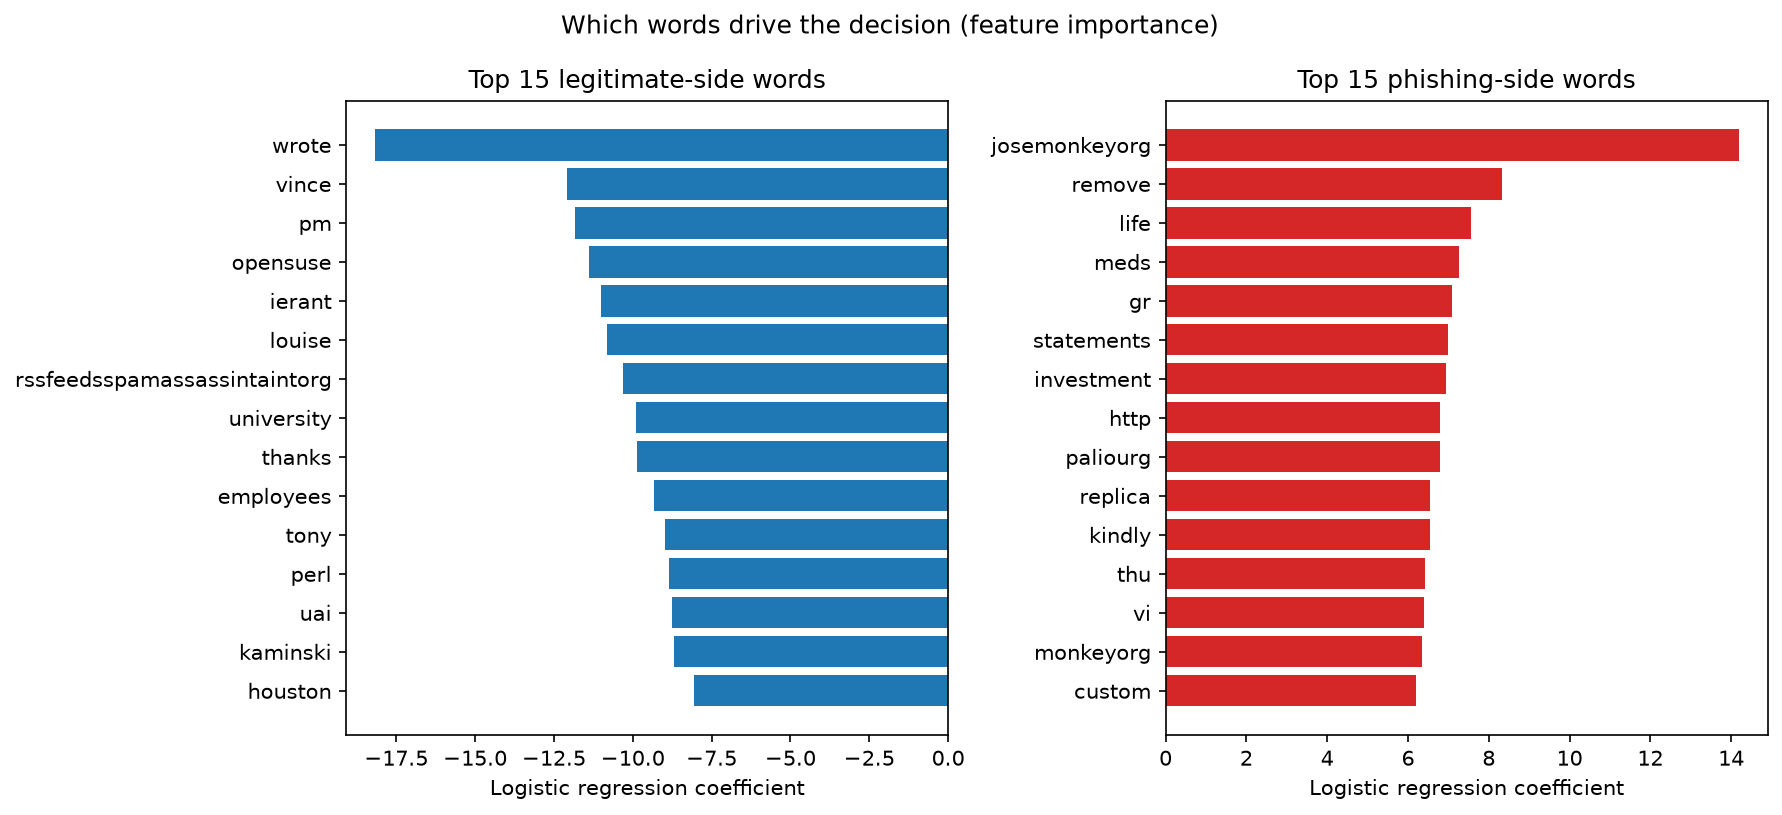
\includegraphics[width=0.85\textwidth]{figs/feature_importance_top_words.png}
\caption{The fifteen strongest words on each side of the decision, read
from the tuned logistic regression coefficients. Alongside genuine
signal, several top features are names of the source archives
themselves.}
\label{fig:importance}
\end{figure*}

\subsection{Limitations}
The scores measure in-distribution separation of the source archives.
A mailbox whose legitimate traffic does not look like Enron-era business
mail --- or whose phishing does not look like archived scams --- would
need retraining and fresh evaluation before any of these numbers could
be promised. Features are unigram TF-IDF only; URL structure was
destroyed upstream and could only be approximated at the token level;
and the labels are inherited from the archives rather than from
per-message review. A cross-source evaluation, where training and
testing draw on different archives, is the natural next measurement.

\section{Conclusion}
We built a phishing email classifier from scratch on an 82{,}486-email
combined corpus, measuring before acting at every step: the
pre-normalisation claim was verified (0.0\% uppercase, 47.2\% URL
tokens), a quantified source watermark was removed (18.2\% vs 0.0\%),
255 extreme outliers were truncated before de-duplication, and the
representation was chosen by a pre-declared tie protocol. Tuned logistic
regression won the four-model comparison with 98.22\% accuracy, F1
0.9829 and the best recall (0.9851, 128 misses in 8{,}569), with the MLP
and random forest within 0.0008 F1 behind. Coefficient inspection showed
the model splits its attention between genuine scam vocabulary and the
names of the archives the corpus was assembled from --- an honest
description of what near-perfect accuracy means here, and a concrete
argument for cross-source evaluation, richer URL features and calibrated
probability outputs as future work.

\section*{Acknowledgment}
This work was carried out during the IICT Summer Internship on AI and
Machine Learning (2026). The author thanks the internship mentor,
Dr.~Ashok, for guidance on the project workflow and requirements.

\begin{thebibliography}{9}

\bibitem{fette2007}
I. Fette, N. Sadeh, and A. Tomasic, ``Learning to detect phishing
emails,'' in \textit{Proc. 16th Int. Conf. on World Wide Web (WWW)},
Banff, Canada, 2007, pp. 649--656.

\bibitem{almomani2013}
A. Almomani, B. B. Gupta, S. Atawneh, A. Meulenberg, and E. Almomani,
``A survey of phishing email filtering techniques,'' \textit{IEEE
Communications Surveys \& Tutorials}, vol. 15, no. 4, pp. 2070--2090,
2013.

\bibitem{klimt2004}
B. Klimt and Y. Yang, ``The Enron corpus: A new dataset for email
classification research,'' in \textit{Proc. European Conf. on Machine
Learning (ECML)}, LNCS vol. 3201, Springer, 2004, pp. 217--226.

\bibitem{metsis2006}
V. Metsis, I. Androutsopoulos, and G. Paliouras, ``Spam filtering with
naive Bayes --- which naive Bayes?'' in \textit{Proc. 3rd Conf. on Email
and Anti-Spam (CEAS)}, Mountain View, CA, USA, 2006.

\bibitem{pedregosa2011}
F. Pedregosa \textit{et al.}, ``Scikit-learn: Machine learning in
Python,'' \textit{Journal of Machine Learning Research}, vol. 12, pp.
2825--2830, 2011.

\end{thebibliography}

\appendix
\section{Reproducibility}
The pipeline is a modular Python project
(\textit{src/data\_loader.py}, \textit{data\_inspection.py},
\textit{data\_cleaning.py}, \textit{text\_preprocessing.py},
\textit{eda.py}, \textit{feature\_engineering.py},
\textit{model\_training.py}, \textit{model\_evaluation.py}) driven by a
single \textit{main.py}. Every figure and number in this paper is
written to disk by the code (\textit{outputs/} and \textit{graphs/});
the fixed seed 42 reproduces the split, the tuning, the features and all
model results exactly. Scikit-learn \cite{pedregosa2011} provides the
learners and vectorizers. The text normalisation applied to every email
is:

\begin{verbatim}
def clean_text(text, stop_words):
    text = text.lower()
    text = URL_PATTERN.sub(" ", text)
    text = HTML_PATTERN.sub(" ", text)
    text = MENTION_PATTERN.sub(" ", text)
    text = NON_LETTER_PATTERN.sub(" ", text)
    words = [w for w in text.split()
             if w not in stop_words
             and len(w) > 1]
    return " ".join(words)
\end{verbatim}

\end{document}
